% A LaTeX template for EXECUTIVE SUMMARY of the MSc Thesis submissions to 
% Politecnico di Milano (PoliMi) - School of Industrial and Information Engineering
%
% S. Bonetti, A. Gruttadauria, G. Mescolini, A. Zingaro
% e-mail: template-tesi-ingind@polimi.it
%
% Last Revision: October 2021
%
% Copyright 2021 Politecnico di Milano, Italy. NC-BY

\documentclass[11pt,a4paper,twocolumn]{article}
\pdfminorversion=7

%------------------------------------------------------------------------------
%	REQUIRED PACKAGES AND CONFIGURATIONS
%------------------------------------------------------------------------------
% PACKAGES FOR TITLES
\usepackage{titlesec}
\usepackage{color}

% PACKAGES FOR LANGUAGE AND FONT
\usepackage[utf8]{inputenc}
\usepackage[english]{babel}
\usepackage[T1]{fontenc} % Font encoding

% PACKAGES FOR IMAGES
\usepackage{graphicx}
\graphicspath{{Images/}} % Path for images' folder
\usepackage{eso-pic} % For the background picture on the title page
\usepackage{subfig} % Numbered and caption subfigures using \subfloat
\usepackage{caption} % Coloured captions
\usepackage{transparent}

% STANDARD MATH PACKAGES
\usepackage{amsmath}
\usepackage{amsthm}
\usepackage{bm}
\usepackage[overload]{empheq}  % For braced-style systems of equations

% PACKAGES FOR TABLES
\usepackage{tabularx}
\usepackage{longtable} % tables that can span several pages
\usepackage{colortbl}

% PACKAGES FOR ALGORITHMS (PSEUDO-CODE)
\usepackage{algorithm}
\usepackage{algorithmic}

% PACKAGES FOR REFERENCES & BIBLIOGRAPHY
\usepackage[colorlinks=true,linkcolor=black,anchorcolor=black,citecolor=black,filecolor=black,menucolor=black,runcolor=black,urlcolor=black]{hyperref} % Adds clickable links at references
\usepackage{cleveref}
\usepackage[square, numbers, sort&compress]{natbib} % Square brackets, citing references with numbers, citations sorted by appearance in the text and compressed
\bibliographystyle{plain} % You may use a different style adapted to your field

% PACKAGES FOR THE APPENDIX
\usepackage{appendix}

% PACKAGES FOR ITEMIZE & ENUMERATES 
\usepackage{enumitem}

% OTHER PACKAGES
\usepackage{amsthm,thmtools,xcolor} % Coloured "Theorem"
\usepackage{comment} % Comment part of code
\usepackage{fancyhdr} % Fancy headers and footers
\usepackage{lipsum} % Insert dummy text
\usepackage{tcolorbox} % Create coloured boxes (e.g. the one for the key-words)
\usepackage{stfloats} % Correct position of the tables

%-------------------------------------------------------------------------
%	NEW COMMANDS DEFINED
%-------------------------------------------------------------------------
\newcommand{\bea}{\begin{eqnarray}} % Shortcut for equation arrays
\newcommand{\eea}{\end{eqnarray}}
\newcommand{\e}[1]{\times 10^{#1}}  % Powers of 10 notation
\newcommand{\mathbbm}[1]{\text{\usefont{U}{bbm}{m}{n}#1}} % From mathbbm.sty
\newcommand{\pdev}[2]{\frac{\partial#1}{\partial#2}}

%----------------------------------------------------------------------------
%	ADD YOUR CONFIGURATION
%----------------------------------------------------------------------------
\input{Configuration_files/config}

% Insert here the info that will be displayed into your Title page 
% -> title of your work
\renewcommand{\title}{Design and Optimization of a High-Performance and Energy-Efficient Branch Predictor in HARCOM}
% -> author name and surname
\renewcommand{\author}{Roberto Di Lauro, Alessandro Ghiotto}
% -> MSc course
\newcommand{\course}{High-Performance Computing Engineering}
% -> advisor name and surname
\newcommand{\advisor}{Marco Ronzani PHD}
% -> co-advisor name and surname
\newcommand{\firstcoadvisor}{Prof. Cristina Silvano} % insert if any otherwise comment
% -> academic year
\newcommand{\YEAR}{2025-2026}

%-------------------------------------------------------------------------
%	BEGIN OF YOUR DOCUMENT
%-------------------------------------------------------------------------
\begin{document}

% This file creates the Title Page of the document
\input{Configuration_files/title_page}

%%%%%%%%%%%%%%%%%%%%%%%%%%%%%%
%%     THESIS MAIN TEXT     %%
%%%%%%%%%%%%%%%%%%%%%%%%%%%%%%

%-----------------------------------------------------------------------------
% INTRODUCTION
%-----------------------------------------------------------------------------
\section{Introduction}
\label{sec:introduction}

In modern high-performance superscalar architectures, exploiting Instruction-Level Parallelism (ILP) relies heavily on the efficiency of the instruction fetch unit. Because deep out-of-order execution pipelines must speculatively fetch and execute instructions across conditional branch boundaries to sustain throughput, any branch misprediction incurs a significant recovery penalty. This penalty involves flushing the pipeline (reorder buffer, reservation stations) and redirecting execution, which severely degrades the Instructions Per Cycle (IPC) and increases energy overhead. Consequently, highly accurate and low-latency branch prediction is a critical design requirement for maximizing execution efficiency.

The objective of this project is to evaluate the trade-offs in branch prediction architectures under tight hardware complexity constraints. Using the Hardware Complexity (\textbf{HARCOM}) library, we perform a comprehensive comparative study of classic branch predictors established in the literature, including global-history-based models (Gshare, GAG, GAP) and local-history-based models (PAG, PAP), alongside their line-wide extensions for block-level prediction. We explore the multi-dimensional design parameter space (varying table configurations, counter widths, and history register lengths) subject to a strict memory budget. The evaluation focuses on maximizing the Voltage-Frequency-Scaled Speedup (\textbf{VFS}) metric~\cite{michaudvfs}, which models the net processor performance by balancing prediction accuracy (Mispredictions Per Kilo-Instruction, or \textbf{MPKI}), hardware \textbf{latency}, and energy consumption (dynamic and static Energy Per Instruction, or \textbf{EPI}). Under the physical timing model in HARCOM, the energy, latency, and area costs of the predictor's logic and memory components are dynamically tracked.

% Specifically, the VFS score evaluates three primary design dimensions:
% \begin{enumerate}
%     \item \textbf{Prediction Accuracy:} Quantified as Mispredictions Per Kilo-Instructions (MPKI), which dictates the rate of wrong-path instruction execution.
%     \item \textbf{Processor Performance (IPC):} Strongly influenced by the latencies of the two prediction stages (Stage 1 and Stage 2) within the instruction fetch pipeline.
%     \item \textbf{Energy Efficiency:} Measured as dynamic and static Energy Per Instruction (EPI) in fJ, dictated by the capacitance, access frequencies, and leakage currents of the predictor's register arrays and SRAM tables.
% \end{enumerate}

% The VFS metric is computed using the CPU speedup ($S$) and the normalized EPI. The processor speedup is defined as:
% \begin{equation}
% \label{eq:speedup}
% S = \frac{\text{IPC}_{\text{cbp}}}{\text{IPC}_{\text{cbp}0}} \times \frac{1 + \text{WPI}_0}{1 + \text{WPI}}
% \end{equation}
% where $\text{WPI} = \text{IPC}_{\text{cbp}} \times \text{CPI}_{\text{cbp}}$ represents the wrong-path instructions per correct-path instruction, and the subscript $0$ indicates the reference core parameters. The normalized energy metric is formulated as:
% \begin{equation}
% \label{eq:epi}
% \begin{split}
% \text{EPI}_{\text{norm}} = {} & \left( \frac{\text{EPI}_{\text{cbp}}}{\text{EPI}_{\text{cbp}0}} \cdot r_{\text{energy}} + \Lambda \cdot S^\Gamma \right) \\
% & \times \left(1 + \frac{\text{WPI}}{2}\right)
% \end{split}
% \end{equation}
% where $r_{\text{energy}} = 0.05$ is the reference energy ratio, $\Lambda = \frac{1}{1 + \text{WPI}_0/2} - r_{\text{energy}}$, and $\Gamma = \frac{2}{\alpha - 1}$ with $\alpha = 1.625$. The final VFS score is derived as:
% \begin{equation}
% \label{eq:vfs}
% \text{VFS} = S \cdot \alpha \left( 1 - \frac{2}{1 + \sqrt{1 + \frac{\beta}{S \cdot \text{EPI}_{\text{norm}}}}} \right)
% \end{equation}
% where $\beta = \frac{4\alpha}{(\alpha - 1)^2}$.

\textcolor{red}{
Building upon this comparative study, we propose a two-stage (two-level) branch predictor variant based on the state-of-the-art \textbf{TAGE}~\cite{seznec2006case} (Tagged Geometric History Length) architecture. TAGE uses multiple tagged predictor tables indexed with geometrically increasing history lengths to capture both short-term path correlations and long-term global context. To adhere to physical timing constraints, our variant decouples the prediction logic into a low-latency Stage 1 helper table for single-cycle fallback decisions and a high-capacity Stage 2 tagged TAGE structure that resolves complex branch histories over two cycles. This design optimizes the trade-off between execution latency, area cost, and accuracy, maximizing the VFS score within the budget limit. Finally, the proposed predictor is validated and evaluated across different instruction traces to assess its performance and robustness under diverse workloads.
}

%-----------------------------------------------------------------------------
% HARCOM FRAMEWORK AND PREDICTOR INTERFACE
%-----------------------------------------------------------------------------
\section{The HARCOM Framework}
\label{sec:harcom}

The simulation environment is built upon the Hardware Complexity (HARCOM) library. In HARCOM, predictors are implemented by inheriting from the \texttt{predictor} structure (a C++ \texttt{struct} that defines the abstract interface). This framework allows modeling physical hardware properties including area, power, and timing by tracking three fundamental data types: \texttt{val<N>}, \texttt{reg<N>} and \texttt{ram<T, N>}.

% \begin{itemize}
%     \item \textbf{\texttt{val<N>}}: Represents an $N$-bit value. Each \texttt{val} dynamically tracks its signal propagation time (latency) as it passes through combinational logic, alongside its dynamic and static energy costs.
%     \item \textbf{\texttt{reg<N>}}: Represents an $N$-bit hardware register, which persists state across clock cycles and is updated once per clock cycle.
%     \item \textbf{\texttt{ram<T, N>}}: Represents a single-port SRAM array of size $N$ with elements of type $T$. To model physical memory constraints, it permits at most one read or one write operation per cycle.
% \end{itemize}

The simulation interface separates the prediction and update processes. To minimize latency overhead on the processor's critical path, the interface supports \textbf{two-stage (two-level) prediction}. In Stage 1 (\texttt{predict1}), a fast, low-latency prediction is generated. In Stage 2 (\texttt{predict2}), a slower but more accurate prediction is computed, overriding the Stage 1 choice if they disagree. 

Furthermore, to support superscalar fetch blocks where multiple instructions are fetched in a single clock cycle, HARCOM enables \textbf{line prediction} (block-level prediction). The first instruction of a block is predicted via \texttt{predict1/2}, which usually performs a big table lookup on the SRAM and store it on the registers, subsequent instructions are predicted via \texttt{reuse\_predict1/2}, by reusing that values we have already loaded. The updates are managed through the \texttt{update\_condbr} method (called after each conditional branch) and the \texttt{update\_cycle} method (called once per block to commit updates). A block ends when we have a taken branch, a misprediction, or when the predictor logic decides that the block ends (call \texttt{reuse\_prediction(0)}). Figure~\ref{fig:harcom-interface} illustrates the flowchart of the interface calls within the simulator.

\begin{figure}[htbp]
    \centering
    
\includegraphics[width=1.0\linewidth]{interface-flowchart}
    \caption{\textbf{Flowchart of the HARCOM predictor interface.}}
    \label{fig:harcom-interface}
\end{figure}

% \section{EDA traces}
% \label{sec:traces}


\section{Experiments}
\label{sec:exploration}

\begin{table*}[tb]
    \caption{\textbf{Chosen training traces.} The following traces where chosen since they are at the extreme of a chosen statistics. \textcolor{red}{\bf{red}} stands for max, \textcolor{blue}{\bf{blue}} for min. The last ones are chosen since they are around the median on some of the statistics. Statistics of the whole train set are in the Appendix.}
    \centering 
    \resizebox{\textwidth}{!}{%
    \begin{tabular}{|lrrrrrrr|}
    \hline
    \rowcolor{bluePoli!40}
    \textbf{trace} & \textbf{\#instr} & \textbf{br density} & \textbf{T rate} & \textbf{BW rate} & \textbf{UC rate} & \textbf{IND rate} & \textbf{\#u cond pc} \\
    \hline \hline
    \texttt{nodejs-misc-util\_7039} & 21,029,395 & \textcolor{red}{\textbf{33.3\%}} & 33.3\% & 33.3\% & 0.0\% & 0.0\% & 274 \\
    \texttt{fp\_28} & 39,000,014 & \textcolor{blue}{\textbf{1.5\%}} & 86.4\% & \textcolor{red}{\textbf{79.7\%}} & 0.7\% & 0.0\% & 40 \\
    \texttt{compress\_44} & 40,000,000 & 24.8\% & \textcolor{red}{\textbf{99.2\%}} & 49.6\% & 0.2\% & 0.0\% & 382 \\
    \texttt{web\_99} & 38,999,990 & 29.0\% & \textcolor{blue}{\textbf{6.5\%}} & 2.6\% & 24.5\% & 0.6\% & 1,080 \\
    \texttt{web\_13} & 38,999,811 & 16.5\% & 31.0\% & 17.5\% & 25.2\% & 12.0\% & \textcolor{red}{\textbf{66,766}} \\ 
    \texttt{infra\_32} & 39,000,014 & 23.6\% & 10.6\% & \textcolor{blue}{\textbf{0.5\%}} & 26.1\% & 12.9\% & 306 \\  
    \texttt{tomcat-wrk2-panel.3289\_0} & 21,128,092 & 17.8\% & 54.1\% & 7.3\% & 37.4\% & \textcolor{red}{\textbf{27.2\%}} & 6,012 \\ 
    \texttt{int\_48} & 39,000,046 & 16.9\% & 39.2\% & 32.7\% & 3.9\% & \textcolor{blue}{\textbf{0.0\%}} & 538 \\
    \texttt{505-mcf-1\_14364} & 21,532,609 & 11.6\% & 39.7\% & 23.3\% & 6.9\% & 0.0\% & 301 \\
    \texttt{compress\_47} & 40,000,000 & 13.3\% & 39.6\% & 28.7\% & 7.7\% & 1.2\% & 1,566 \\
    \texttt{int\_210} & 39,000,050 & 15.4\% & 41.9\% & 17.9\% & 15.4\% & 4.0\% & 1,170 \\
    \texttt{java16-specjbb-4k.23837\_0} & 21,044,473 & 13.6\% & 43.0\% & 14.0\% & 24.0\% & 10.3\% & 493 \\
    \hline
    \end{tabular}%
    }
    \label{table:chosen-traces}
\end{table*}


We started by implementing and evaluating the standard predictors from the literature under two memory budgets: \textbf{8 KB} and \textbf{16 KB}.
% These budgets are highly representative: 8 KB aligns with standard academic benchmarks (e.g., Championship Branch Prediction low-power track) for high-efficiency embedded cores, while 16 KB represents the critical physical transition threshold in HARCOM where memory latency scaling begins to dominate branch predictor performance. 
As traces we have chosen 12 across 168 CBP-NG training traces. We have chosen them by looking at the statistics of the traces, in particular by taking the ones which are at the extremes of some of such statistics. 
% For example we have chosen the traces with highest and lowest branch density, conditional taken rate, backward rate, indirect rate, max number of unique PCs, and some examples which instead are around the median. 
The chosen trace informations can be seen in Table~\ref{table:chosen-traces}.
For each family, we swept parameters trading table capacity for indexing accuracy, by varying mainly the global history length (\texttt{BHR\_B}) and PC bits (\texttt{PC\_B}), which define the size of the PHT. 
% global history length (\texttt{BHR\_B}), PC bits (\texttt{PC\_B}); LHT entries (\texttt{LOG\_GHT}/\texttt{PC\_B}) and local history (\texttt{BHR\_B}) for \texttt{pagL}, \texttt{papL} (adding PHT PC bits \texttt{PC\_B2}), and \texttt{lxorL}; and Choice (\texttt{LOG\_CHOICE}) vs. Direction (\texttt{LOG\_PHT}) table sizes for \texttt{bimodeL}. Table~\ref{table:budget_comparison} (located on page 3) summarizes the optimal configurations.

\begin{table}[htbp]
    \caption{\textbf{Performance Summary.} Average across the 12 traces of all metrics, on the best predictors. All the results are in Table~\ref{table:block_avg_performance}.}
    \centering
    \resizebox{\columnwidth}{!}{%
    \begin{tabular}{|lrrrrr|}
    \hline
    \rowcolor{bluePoli!40}
    \textbf{Predictor} & \textbf{Budget} & \textbf{VFS} & \textbf{MPKI} & \textbf{IPC} & \textbf{EPI} \T\B \\
    \hline \hline
    \texttt{tage\bf{L}}       & 8 KB  & \textbf{0.7101} & 5.80 & \textbf{4.7806} & 939.6 \\
    \texttt{tage\bf{L}}       & 16 KB & 0.6988 & 5.42 & 4.7048 & 1145.5 \\
    \texttt{tage\_u\bf{L}}    & 8 KB  & 0.6727 & 4.62 & 4.3510 & 821.8 \\
    \texttt{tage\_u\bf{L}}    & 16 KB & 0.6666 & \textbf{4.19} & 4.2656 & 933.4 \\
    \texttt{gshare\bf{L}}     & 8 KB  & 0.6544 & 5.25 & 3.4839 & \textbf{115.8} \\
    \texttt{gshare\bf{L}}     & 16 KB & 0.6586 & 4.93 & 3.4934 & 145.5 \\
    \hline
    \texttt{gap}         & 8 KB  & \textbf{0.2338} & 6.32 & \textbf{0.9898} & \textbf{217.9} \\
    \texttt{tage}        & 8 KB  & 0.2254 & 5.49 & 0.9846 & 1662.2 \\
    \texttt{tage}        & 16 KB & 0.2239 & \textbf{5.01} & 0.9851 & 2401.2 \\
    \texttt{gshare}      & 16 KB & 0.1219 & 5.07 & 0.4979 & 263.2 \\
    \hline
    \end{tabular}%
    }
    \label{table:compact_summary}
\end{table}

\subsection{Experimental Results and Design Space Analysis}
Analyzing the simulation data (summarized for key configurations in Table~\ref{table:compact_summary}) reveals several insights into the trade-offs of branch predictor design:

\textbf{Trace Characteristics and Predictor Suitability:} Simple global-history predictors (\texttt{gshareL}, \texttt{gapL}, and \texttt{gagL}) perform exceptionally well on traces with low branch complexity. For instance, on \texttt{fp\_28} (which has a low branch density of 1.5\% and only 40 unique conditional PCs), \texttt{gshareL} achieves a high VFS score of 1.034, since aliasing in the prediction tables is negligible. Conversely, on complex workloads like \texttt{web\_13} (which contains 66,766 unique conditional PCs), the tagged geometric history length (\texttt{tageL}, \texttt{tage\_uL}) predictors outperform them significantly (VFS of 0.756 for \texttt{tageL} vs. 0.655 for \texttt{gshareL}). Tagged components successfully mitigate destructive aliasing across huge branch working sets. For traces with extremely high indirect rates (such as \texttt{tomcat-wrk2-panel.3289\_0} at 27.2\%), all conditional branch predictors suffer a general performance degradation due to the indirect branch recovery penalties.

\textbf{Block vs. Scalar Predictors:} Block-level predictors (suffix \texttt{L}) fetch and predict multiple instructions in a single cycle by reusing the active SRAM row, leading to an IPC range of 3.0--4.7, compared to only 0.49--0.98 for scalar models. More importantly, this throughput dominance translates directly into energy efficiency: block predictors achieve VFS speedup factors of 3.0x--5.64x over their scalar counterparts. The amortized Energy Per Instruction (EPI) remains highly competitive, proving that line-wide prediction is crucial for high-performance out-of-order cores.

\textbf{Predictor Groups and Behaviors:} The global-indexed models (\texttt{gap}, \texttt{gag}, and \texttt{gshare}) behave very similarly, as they use variations of global history XORed or concatenated with the PC address, yielding clustered VFS and MPKI scores (e.g., VFS of 0.6586, 0.6525, 0.6472 respectively at 16 KB block). When comparing TAGE variants, \texttt{tageL} achieves a higher IPC (4.7048 vs. 4.2656) due to simpler update rules, whereas \texttt{tage\_uL} achieves a lower MPKI (4.19 vs. 5.42) by utilizing usefulness (\texttt{u}) bits to track and deallocate useless entries, highlighting the accuracy-throughput trade-off.

\textbf{The 16 KB vs. 8 KB Budget Trade-off:} Doubling the budget from 8 KB to 16 KB consistently reduces the branch misprediction rate (e.g., \texttt{gshareL} MPKI drops from 5.25 to 4.93). However, under HARCOM's physical timing and energy model, a larger budget is not guaranteed to improve the VFS score. Higher capacity increases SRAM access latency and dynamic/static energy (e.g., \texttt{tageL} EPI increases from 939.6 fJ at 8 KB to 1145.5 fJ at 16 KB). As a result, the average VFS score for several predictors actually degrades when moving from 8 KB to 16 KB (e.g., \texttt{tageL} VFS drops from 0.7101 to 0.6988).

\begin{table*}[htbp]
    \caption{\textbf{Block Predictor VFS Scores Per Trace Breakdown (8 KB Budget)}}
    \centering
    \resizebox{\textwidth}{!}{%
    \begin{tabular}{|lcccccccccccc|c|}
    \hline
    \rowcolor{bluePoli!40}
    \textbf{Predictor} & \textbf{505-mcf} & \textbf{compr4} & \textbf{compr7} & \textbf{fp} & \textbf{infra} & \textbf{int} & \textbf{int} & \textbf{specjbb} & \textbf{nodejs} & \textbf{tomcat} & \textbf{web} & \textbf{web} & \textbf{Mean} \T\B \\
    \hline \hline
    \texttt{tageL} & 0.724 & \textbf{0.596} & \textbf{0.765} & 0.749 & \textbf{0.873} & \textbf{0.546} & \textbf{0.706} & \textbf{0.813} & 0.524 & \textbf{0.615} & \textbf{0.756} & \textbf{0.854} & \textbf{0.710} \\
    \texttt{tage\_uL} & \textbf{0.728} & 0.490 & 0.755 & 0.742 & 0.863 & 0.524 & 0.631 & 0.766 & 0.449 & 0.580 & 0.699 & 0.845 & \textbf{0.673} \\
    \texttt{gshareL} & 0.704 & 0.330 & 0.755 & \textbf{1.034} & 0.738 & 0.535 & 0.691 & 0.719 & \textbf{0.541} & 0.526 & 0.655 & 0.625 & \textbf{0.654} \\
    \texttt{gapL} & 0.687 & 0.330 & 0.755 & \textbf{1.034} & 0.729 & 0.532 & 0.681 & 0.713 & \textbf{0.541} & 0.525 & 0.642 & 0.601 & \textbf{0.647} \\
    \texttt{gagL} & 0.705 & 0.330 & 0.755 & 1.033 & 0.707 & 0.527 & 0.686 & 0.719 & \textbf{0.541} & 0.501 & 0.627 & 0.583 & \textbf{0.643} \\
    \texttt{bimodeL} & 0.672 & 0.324 & 0.734 & 1.033 & 0.734 & 0.510 & 0.659 & 0.694 & 0.533 & 0.540 & 0.650 & 0.615 & \textbf{0.641} \\
    \texttt{papL} & 0.646 & 0.327 & 0.657 & 1.032 & 0.720 & 0.432 & 0.615 & 0.707 & 0.538 & 0.480 & 0.600 & 0.581 & \textbf{0.611} \\
    \texttt{pagL} & 0.652 & 0.325 & 0.640 & 1.030 & 0.710 & 0.405 & 0.600 & 0.705 & 0.535 & 0.457 & 0.580 & 0.564 & \textbf{0.600} \\
    \texttt{lxorL} & 0.624 & 0.325 & 0.651 & 1.032 & 0.698 & 0.386 & 0.593 & 0.699 & 0.535 & 0.455 & 0.583 & 0.557 & \textbf{0.595} \\
    \texttt{percL\_16} & 0.417 & 0.164 & 0.436 & 0.775 & 0.411 & 0.305 & 0.367 & 0.393 & 0.275 & 0.287 & 0.344 & 0.333 & \textbf{0.376} \\
    \texttt{percL\_4} & 0.344 & 0.245 & 0.362 & 0.466 & 0.393 & 0.303 & 0.350 & 0.362 & 0.365 & 0.309 & 0.334 & 0.370 & \textbf{0.350} \\
    \hline
    \end{tabular}%
    }
    \label{table:block_8kb_vfs}
\end{table*}

\begin{table*}[htbp]
    \caption{\textbf{Block Predictor VFS Scores Per Trace Breakdown (16 KB Budget)}}
    \centering
    \resizebox{\textwidth}{!}{%
    \begin{tabular}{|lcccccccccccc|c|}
    \hline
    \rowcolor{bluePoli!40}
    \textbf{Predictor} & \textbf{505-mcf} & \textbf{compr4} & \textbf{compr7} & \textbf{fp} & \textbf{infra} & \textbf{int} & \textbf{int} & \textbf{specjbb} & \textbf{nodejs} & \textbf{tomcat} & \textbf{web} & \textbf{web} & \textbf{Mean} \T\B \\
    \hline \hline
    \texttt{tageL} & 0.701 & \textbf{0.590} & 0.747 & 0.764 & \textbf{0.861} & 0.532 & 0.685 & \textbf{0.788} & 0.521 & \textbf{0.613} & \textbf{0.747} & 0.837 & \textbf{0.699} \\
    \texttt{tage\_uL} & \textbf{0.727} & 0.375 & \textbf{0.755} & 0.762 & 0.855 & 0.539 & 0.598 & 0.783 & 0.448 & 0.585 & 0.724 & \textbf{0.848} & \textbf{0.667} \\
    \texttt{gshareL} & 0.711 & 0.329 & 0.754 & 1.033 & 0.739 & \textbf{0.551} & \textbf{0.693} & 0.721 & \textbf{0.540} & 0.546 & 0.662 & 0.624 & \textbf{0.659} \\
    \texttt{gapL} & 0.702 & 0.329 & \textbf{0.755} & \textbf{1.034} & 0.729 & 0.545 & 0.689 & 0.719 & \textbf{0.540} & 0.539 & 0.647 & 0.602 & \textbf{0.653} \\
    \texttt{gagL} & 0.712 & 0.329 & 0.754 & 1.033 & 0.707 & 0.543 & 0.687 & 0.721 & \textbf{0.540} & 0.516 & 0.633 & 0.592 & \textbf{0.647} \\
    \texttt{bimodeL} & 0.683 & 0.323 & 0.734 & 1.032 & 0.734 & 0.523 & 0.666 & 0.698 & 0.532 & 0.550 & 0.651 & 0.615 & \textbf{0.645} \\
    \texttt{papL} & 0.644 & 0.326 & 0.658 & 1.031 & 0.724 & 0.439 & 0.613 & 0.704 & 0.537 & 0.472 & 0.582 & 0.583 & \textbf{0.610} \\
    \texttt{lxorL} & 0.624 & 0.325 & 0.651 & 1.032 & 0.698 & 0.386 & 0.593 & 0.699 & 0.535 & 0.455 & 0.583 & 0.557 & \textbf{0.595} \\
    \texttt{pagL} & 0.663 & 0.325 & 0.619 & 1.029 & 0.612 & 0.370 & 0.590 & 0.618 & 0.538 & 0.395 & 0.528 & 0.518 & \textbf{0.567} \\
    \texttt{percL\_16} & 0.416 & 0.164 & 0.435 & 0.774 & 0.409 & 0.304 & 0.365 & 0.391 & 0.274 & 0.288 & 0.342 & 0.332 & \textbf{0.375} \\
    \texttt{percL\_4} & 0.339 & 0.241 & 0.356 & 0.460 & 0.388 & 0.300 & 0.345 & 0.357 & 0.359 & 0.309 & 0.330 & 0.364 & \textbf{0.346} \\
    \hline
    \end{tabular}%
    }
    \label{table:block_16kb_vfs}
\end{table*}

\clearpage

%---------------------------------------------------------------------------
%  APPENDIX
%---------------------------------------------------------------------------
\appendix
\section{Trace Characteristics}
\label{sec:appendix_traces}

\begin{table*}[tb]
    \caption{\textbf{Statistics of the training traces.} Min, Max and Quartiles at 0.25, 0.5 and 0.75 over the whole dataset of training traces, on the chosen statistics.}
    \centering 
    \begin{tabular}{|lrrrrr|}
    \hline
    \rowcolor{bluePoli!40}
    & \textbf{Min} & \textbf{Q1} & \textbf{Q2} & \textbf{Q3} & \textbf{Max} \\
    \hline \hline
    br density & 1.5\% & 15.3\% & 18.8\% & 20.6\% & 33.3\% \\
    cond taken rate & 6.4\% & 33.2\% & 39.6\% & 45.8\% & 99.2\% \\
    backward rate & 0.4\% & 10.6\% & 14.8\% & 23.0\% & 79.6\% \\
    unique cond PCs & 40 & 567 & 1,553 & 10,422 & 66,766 \\
    indirect rate & 0.0\% & 2.7\% & 8.7\% & 14.5\% & 27.2\% \\
    \hline
    \end{tabular}
    % \\[10pt]
    % \caption{Min, Max and Quartiles at 0.25, 0.5 and 0.75 over the whole dataset of training traces, on the chosen statistics.}
    \label{table:traces}
\end{table*}

\section{Extended Simulation Results}
\label{sec:appendix_results}

This section presents the complete breakdown of VFS scores for both Block and Scalar predictors across the 12 representative traces, followed by the predictor family speedups and VFS comparison plots.

% \begin{table*}[htbp]
%     \caption{\textbf{Scalar Predictor VFS Scores Per Trace Breakdown (8 KB Budget)}}
%     \centering
%     \resizebox{\textwidth}{!}{%
%     \begin{tabular}{|lcccccccccccc|c|}
%     \hline
%     \rowcolor{bluePoli!40}
%     \textbf{Predictor} & \textbf{505-mcf-1} & \textbf{compress} & \textbf{compress} & \textbf{fp} & \textbf{infra} & \textbf{int} & \textbf{int} & \textbf{specjbb} & \textbf{nodejs} & \textbf{tomcat} & \textbf{web} & \textbf{web} & \textbf{Mean} \T\B \\
%     \hline \hline
%     \texttt{gap} & 0.2187 & 0.2480 & 0.2338 & 0.2461 & 0.2422 & 0.2093 & 0.2289 & 0.2359 & 0.2487 & 0.2274 & 0.2290 & 0.2378 & \textbf{0.2338} \\
%     \texttt{tage\_simple} & 0.2110 & 0.2394 & 0.2220 & 0.2372 & 0.2342 & 0.1999 & 0.2232 & 0.2313 & 0.2401 & 0.2134 & 0.2199 & 0.2334 & \textbf{0.2254} \\
%     \texttt{gshare} & 0.1199 & 0.1251 & 0.1212 & 0.1245 & 0.1234 & 0.1154 & 0.1215 & 0.1236 & 0.1253 & 0.1182 & 0.1202 & 0.1234 & \textbf{0.1218} \\
%     \texttt{gag} & 0.1200 & 0.1251 & 0.1212 & 0.1244 & 0.1172 & 0.1150 & 0.1213 & 0.1236 & 0.1253 & 0.1162 & 0.1189 & 0.1211 & \textbf{0.1208} \\
%     \texttt{bimode} & 0.1176 & 0.1240 & 0.1200 & 0.1234 & 0.1225 & 0.1142 & 0.1196 & 0.1211 & 0.1242 & 0.1193 & 0.1195 & 0.1224 & \textbf{0.1206} \\
%     \texttt{pap} & 0.1170 & 0.1244 & 0.1180 & 0.1238 & 0.1229 & 0.1115 & 0.1178 & 0.1221 & 0.1247 & 0.1164 & 0.1178 & 0.1221 & \textbf{0.1199} \\
%     \texttt{perceptron} & 0.1171 & 0.1228 & 0.1195 & 0.1223 & 0.1214 & 0.1140 & 0.1189 & 0.1213 & 0.1229 & 0.1174 & 0.1175 & 0.1216 & \textbf{0.1197} \\
%     \texttt{lxor} & 0.1164 & 0.1245 & 0.1179 & 0.1238 & 0.1228 & 0.1099 & 0.1172 & 0.1215 & 0.1247 & 0.1156 & 0.1179 & 0.1217 & \textbf{0.1195} \\
%     \texttt{tage\_simple\_u} & 0.1170 & 0.1224 & 0.1183 & 0.1221 & 0.1210 & 0.1136 & 0.1179 & 0.1202 & 0.1225 & 0.1172 & 0.1185 & 0.1214 & \textbf{0.1193} \\
%     \texttt{pag} & 0.1140 & 0.1239 & 0.1165 & 0.1231 & 0.1223 & 0.1107 & 0.1166 & 0.1212 & 0.1241 & 0.1169 & 0.1177 & 0.1214 & \textbf{0.1190} \\
%     \hline
%     \end{tabular}%
%     }
%     \label{table:scalar_8kb_vfs}
% \end{table*}

% \begin{table*}[htbp]
%     \caption{\textbf{Scalar Predictor VFS Scores Per Trace Breakdown (16 KB Budget)}}
%     \centering
%     \resizebox{\textwidth}{!}{%
%     \begin{tabular}{|lcccccccccccc|c|}
%     \hline
%     \rowcolor{bluePoli!40}
%     \textbf{Predictor} & \textbf{505-mcf-1} & \textbf{compress} & \textbf{compress} & \textbf{fp} & \textbf{infra} & \textbf{int} & \textbf{int} & \textbf{specjbb} & \textbf{nodejs} & \textbf{tomcat} & \textbf{web} & \textbf{web} & \textbf{Mean} \T\B \\
%     \hline \hline
%     \texttt{tage\_simple} & 0.2095 & 0.2368 & 0.2198 & 0.2346 & 0.2316 & 0.2010 & 0.2219 & 0.2288 & 0.2375 & 0.2152 & 0.2195 & 0.2311 & \textbf{0.2239} \\
%     \texttt{gshare} & 0.1198 & 0.1249 & 0.1211 & 0.1243 & 0.1234 & 0.1162 & 0.1216 & 0.1234 & 0.1251 & 0.1197 & 0.1203 & 0.1235 & \textbf{0.1219} \\
%     \texttt{gap} & 0.1185 & 0.1250 & 0.1214 & 0.1244 & 0.1225 & 0.1150 & 0.1209 & 0.1225 & 0.1252 & 0.1177 & 0.1195 & 0.1220 & \textbf{0.1212} \\
%     \texttt{gag} & 0.1199 & 0.1249 & 0.1211 & 0.1242 & 0.1174 & 0.1157 & 0.1212 & 0.1234 & 0.1251 & 0.1170 & 0.1190 & 0.1214 & \textbf{0.1209} \\
%     \texttt{bimode} & 0.1178 & 0.1237 & 0.1198 & 0.1231 & 0.1223 & 0.1145 & 0.1196 & 0.1215 & 0.1239 & 0.1197 & 0.1192 & 0.1222 & \textbf{0.1206} \\
%     \texttt{pap} & 0.1170 & 0.1244 & 0.1179 & 0.1237 & 0.1228 & 0.1117 & 0.1178 & 0.1220 & 0.1246 & 0.1166 & 0.1177 & 0.1220 & \textbf{0.1199} \\
%     \texttt{perceptron} & 0.1169 & 0.1225 & 0.1193 & 0.1221 & 0.1212 & 0.1141 & 0.1187 & 0.1211 & 0.1227 & 0.1180 & 0.1175 & 0.1213 & \textbf{0.1196} \\
%     \texttt{lxor} & 0.1161 & 0.1241 & 0.1176 & 0.1235 & 0.1225 & 0.1100 & 0.1173 & 0.1212 & 0.1243 & 0.1163 & 0.1183 & 0.1216 & \textbf{0.1194} \\
%     \texttt{pag} & 0.1136 & 0.1238 & 0.1170 & 0.1230 & 0.1221 & 0.1107 & 0.1164 & 0.1212 & 0.1241 & 0.1179 & 0.1180 & 0.1213 & \textbf{0.1191} \\
%     \texttt{tage\_simple\_u} & 0.1161 & 0.1214 & 0.1177 & 0.1211 & 0.1199 & 0.1137 & 0.1172 & 0.1191 & 0.1167 & 0.1179 & 0.1179 & 0.1204 & \textbf{0.1183} \\
%     \hline
%     \end{tabular}%
%     }
%     \label{table:scalar_16kb_vfs}
% \end{table*}


\begin{table*}[htbp]
    \caption{\textbf{Block Predictor Average Performance across 12 Traces.} Here we can see the average over the traces of the predictor, on VFS (Voltage-Frequency-Scaled Speedup), MPKI (Mispredictions Per Kilo Instruction), IPC (Instruction Per Clock cycle) and EPI (Energy Per Instruction). Seeing all the metrics allows us to understand better the pros and cons of each predictor.}
    \centering
    \resizebox{\textwidth}{!}{%
    \begin{tabular}{|l c l c c c c|}
    \hline
    \rowcolor{bluePoli!40}
    \textbf{Predictor} & \textbf{Budget} & \textbf{Configuration Template} & \textbf{VFS} & \textbf{MPKI} & \textbf{IPC} & \textbf{EPI} \T\B \\
    \hline \hline
    \texttt{tageL} & 16KB & \texttt{tage\_simpleL<9,16,64,4,16,64,3,4>} & \textbf{0.6988} & 5.42 & \textbf{4.7048} & 1145.5 \\
    \texttt{tage\_uL} & 16KB & \texttt{tage\_simple\_uL<9,16,64,4,16,64,3,4>} & 0.6666 & \textbf{4.19} & 4.2656 & 933.4 \\
    \texttt{gshareL} & 16KB & \texttt{gshare\_simpleL<12,12,2,4>} & 0.6586 & 4.93 & 3.4934 & \textbf{145.5} \\
    \texttt{gapL} & 16KB & \texttt{gapL<10,2,2,4>} & 0.6525 & 5.28 & 3.4829 & \textbf{143.5} \\
    \texttt{gagL} & 16KB & \texttt{gagL<12,2,4>} & 0.6472 & 5.65 & 3.4750 & \textbf{144.1} \\
    \texttt{bimodeL} & 16KB & \texttt{bimodeL<11,12,10,2,4>} & 0.6452 & 4.90 & 3.4168 & 414.5 \\
    \texttt{papL} & 16KB & \texttt{papL<8,10,3,2,4>} & 0.6096 & 6.82 & 3.2616 & 255.5 \\
    \texttt{lxorL} & 16KB & \texttt{lxorL<12,5,4>} & 0.5948 & 8.31 & 3.2719 & 349.9 \\
    \texttt{pagL} & 16KB & \texttt{pagL<12,2,2,4>} & 0.5672 & 8.93 & 3.0710 & 240.8 \\
    \texttt{perceptronL\_LI16} & 16KB & \texttt{perceptron\_simpleL<8,3,8,83,4>} & 0.3746 & 6.91 & 1.7369 & 653.9 \\
    \texttt{perceptronL\_LI4} & 16KB & \texttt{perceptron\_simpleL<9,7,8,83,2>} & 0.3457 & 5.52 & 1.5510 & 1119.2 \\
    \hline
    \texttt{tageL} & 8KB & \texttt{tage\_simpleL<8,16,64,4,16,64,3,4>} & \textbf{0.7101} & 5.80 & \textbf{4.7806} & 939.6 \\
    \texttt{tage\_uL} & 8KB & \texttt{tage\_simple\_uL<8,15,64,4,16,64,3,4>} & 0.6727 & \textbf{4.62} & 4.3510 & 821.8 \\
    \texttt{gshareL} & 8KB & \texttt{gshare\_simpleL<11,11,2,4>} & 0.6544 & 5.25 & 3.4839 & \textbf{115.8} \\
    \texttt{gapL} & 8KB & \texttt{gapL<9,2,2,4>} & 0.6474 & 5.64 & 3.4719 & \textbf{114.1} \\
    \texttt{gagL} & 8KB & \texttt{gagL<11,2,4>} & 0.6429 & 5.99 & 3.4659 & \textbf{114.4} \\
    \texttt{bimodeL} & 8KB & \texttt{bimodeL<10,10,9,2,4>} & 0.6415 & 5.19 & 3.4106 & 375.3 \\
    \texttt{papL} & 8KB & \texttt{papL<8,12,2,2,4>} & 0.6111 & 6.75 & 3.2641 & 243.9 \\
    \texttt{pagL} & 8KB & \texttt{pagL<10,11,2,4>} & 0.6002 & 7.47 & 3.2392 & 350.2 \\
    \texttt{lxorL} & 8KB & \texttt{lxorL<12,5,4>} & 0.5948 & 8.31 & 3.2719 & 349.9 \\
    \texttt{perceptronL\_LI16} & 8KB & \texttt{perceptron\_simpleL<7,3,8,83,4>} & 0.3756 & 6.99 & 1.7378 & 543.2 \\
    \texttt{perceptronL\_LI4} & 8KB & \texttt{perceptron\_simpleL<8,7,8,83,2>} & 0.3502 & 5.67 & 1.5506 & 562.5 \\
    \hline
    \end{tabular}%
    }
    \label{table:block_avg_performance}
\end{table*}

\begin{table*}[htbp]
    \caption{\textbf{Scalar Predictor Average Performance across 12 Traces.} As Table~\ref{table:block_avg_performance} but for the scalar versions. Compering this two tables allows to see in particular that the block based predictors gives a massive boost in IPC and EPI (as expected).}
    \centering
    \resizebox{\textwidth}{!}{%
    \begin{tabular}{|l c l c c c c|}
    \hline
    \rowcolor{bluePoli!40}
    \textbf{Predictor} & \textbf{Budget} & \textbf{Configuration Template} & \textbf{VFS} & \textbf{MPKI} & \textbf{IPC} & \textbf{EPI} \T\B \\
    \hline \hline
    \texttt{tage} & 16KB & \texttt{tage\_simple<11,17,64,4,16,64,3>} & \textbf{0.2239} & 5.01 & \textbf{0.9851} & 2401.2 \\
    \texttt{gshare} & 16KB & \texttt{gshare\_simple<16,16,2>} & 0.1219 & 5.07 & 0.4979 & \textbf{263.2} \\
    \texttt{gap} & 16KB & \texttt{gap<10,6,2>} & 0.1212 & 6.26 & 0.4974 & \textbf{257.5} \\
    \texttt{gag} & 16KB & \texttt{gag<16,2>} & 0.1209 & 6.82 & 0.4972 & \textbf{259.5} \\
    \texttt{bimode} & 16KB & \texttt{bimode<15,14,14,2>} & 0.1206 & 4.68 & 0.4964 & 694.2 \\
    \texttt{pap} & 16KB & \texttt{pap<8,10,7,2>} & 0.1199 & 6.00 & 0.4931 & 421.8 \\
    \texttt{perceptron} & 16KB & \texttt{perceptron\_simple<10,15,8,83>} & 0.1196 & 4.68 & 0.4974 & 1368.6 \\
    \texttt{lxor} & 16KB & \texttt{lxor<11,7>} & 0.1194 & 6.67 & 0.4937 & 526.7 \\
    \texttt{pag} & 16KB & \texttt{pag<15,12,2>} & 0.1191 & 6.08 & 0.4921 & 628.3 \\
    \texttt{tage\_u} & 16KB & \texttt{tage\_simple\_u<11,16,64,4,16,64,3>} & 0.1183 & \textbf{3.46} & 0.4930 & 2047.4 \\
    \hline
    \texttt{\textbf{gap}} & 8KB & \texttt{gap<5,10,2>} & \textbf{0.2338} & 6.32 & \textbf{0.9898} & \textbf{217.9} \\
    \texttt{tage} & 8KB & \texttt{tage\_simple<10,17,64,4,16,64,3>} & 0.2254 & 5.49 & \textbf{0.9846} & 1662.2 \\
    \texttt{gshare} & 8KB & \texttt{gshare\_simple<15,15,2>} & 0.1218 & 5.53 & 0.4977 & \textbf{224.6} \\
    \texttt{gag} & 8KB & \texttt{gag<15,2>} & 0.1208 & 7.24 & 0.4970 & \textbf{221.0} \\
    \texttt{bimode} & 8KB & \texttt{bimode<14,12,13,2>} & 0.1206 & 5.03 & 0.4964 & 596.7 \\
    \texttt{pap} & 8KB & \texttt{pap<8,10,6,2>} & 0.1199 & 6.08 & 0.4931 & 405.2 \\
    \texttt{perceptron} & 8KB & \texttt{perceptron\_simple<9,15,8,83>} & 0.1197 & 4.88 & 0.4973 & 1220.2 \\
    \texttt{lxor} & 8KB & \texttt{lxor<10,7>} & 0.1195 & 7.03 & 0.4934 & 401.3 \\
    \texttt{tage\_u} & 8KB & \texttt{tage\_simple\_u<10,16,64,4,16,64,3>} & 0.1193 & \textbf{3.93} & 0.4944 & 1354.0 \\
    \texttt{pag} & 8KB & \texttt{pag<14,11,2>} & 0.1190 & 6.32 & 0.4921 & 590.3 \\
    \hline
    \end{tabular}%
    }
    \label{table:scalar_avg_performance}
\end{table*}



\begin{figure*}[htbp]

    \centering

    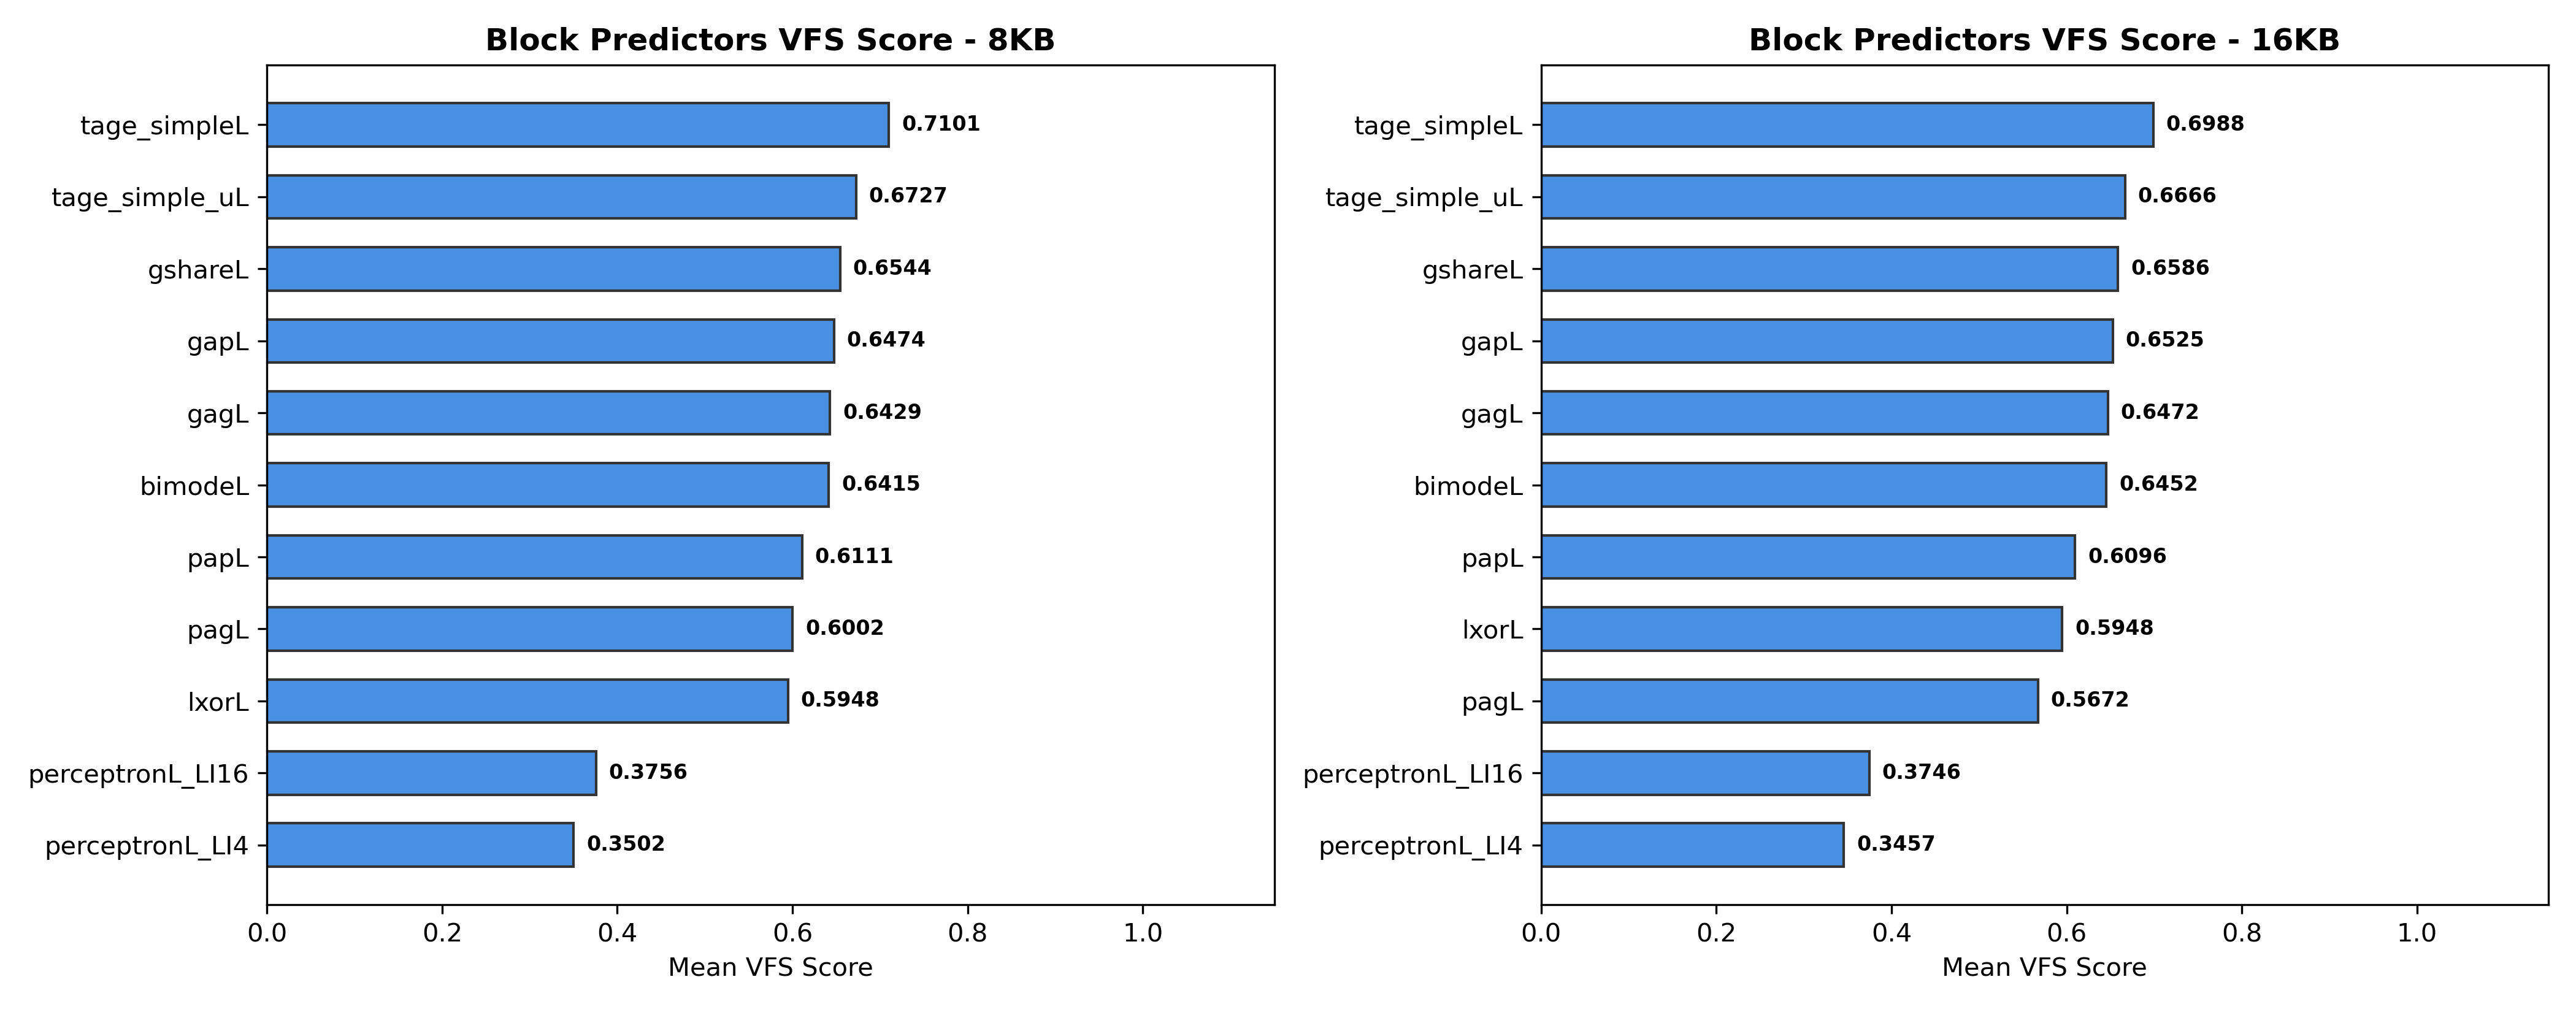
\includegraphics[width=0.95\textwidth]{block_vfs_comparison}

    \caption{\textbf{Block Predictor VFS Score Comparison across 8 KB and 16 KB Budgets.}}

    \label{fig:block_vfs_comparison}

\end{figure*}

\begin{table}[htbp]
    \caption{\textbf{Block vs. Scalar Predictor Family VFS Performance Speedup}}
    \centering
    \resizebox{\columnwidth}{!}{%
    \begin{tabular}{|l c c|}
    \hline
    \rowcolor{bluePoli!40}
    \textbf{Predictor Family} & \textbf{Budget} & \textbf{Speedup Ratio} \T\B \\
    \hline \hline
    \textbf{TAGE\_U}    & 8 KB  & \textbf{5.64x} \\
                        & 16 KB & \textbf{5.64x} \\
    \hline
    \textbf{GShare}     & 8 KB  & \textbf{5.37x} \\
                        & 16 KB & \textbf{5.40x} \\
    \hline
    \textbf{GAg}        & 8 KB  & \textbf{5.32x} \\
                        & 16 KB & \textbf{5.35x} \\
    \hline
    \textbf{BiMode}     & 8 KB  & \textbf{5.32x} \\
                        & 16 KB & \textbf{5.35x} \\
    \hline
    \textbf{PAp}        & 8 KB  & \textbf{5.10x} \\
                        & 16 KB & \textbf{5.09x} \\
    \hline
    \textbf{PAg}        & 8 KB  & \textbf{5.04x} \\
                        & 16 KB & \textbf{4.76x} \\
    \hline
    \textbf{LXOR}       & 8 KB  & \textbf{4.98x} \\
                        & 16 KB & \textbf{4.98x} \\
    \hline
    \textbf{TAGE}       & 8 KB  & \textbf{3.15x} \\
                        & 16 KB & \textbf{3.12x} \\
    \hline
    \textbf{Perceptron} & 8 KB  & \textbf{3.03x} \\
                        & 16 KB & \textbf{3.01x} \\
    \hline
    \textbf{GAp}        & 8 KB  & \textbf{2.77x} \\
                        & 16 KB & \textbf{5.38x} \\
    \hline
    \end{tabular}%
    }
    \label{table:family_speedup}
\end{table}

\begin{figure}[htbp]
    \centering
    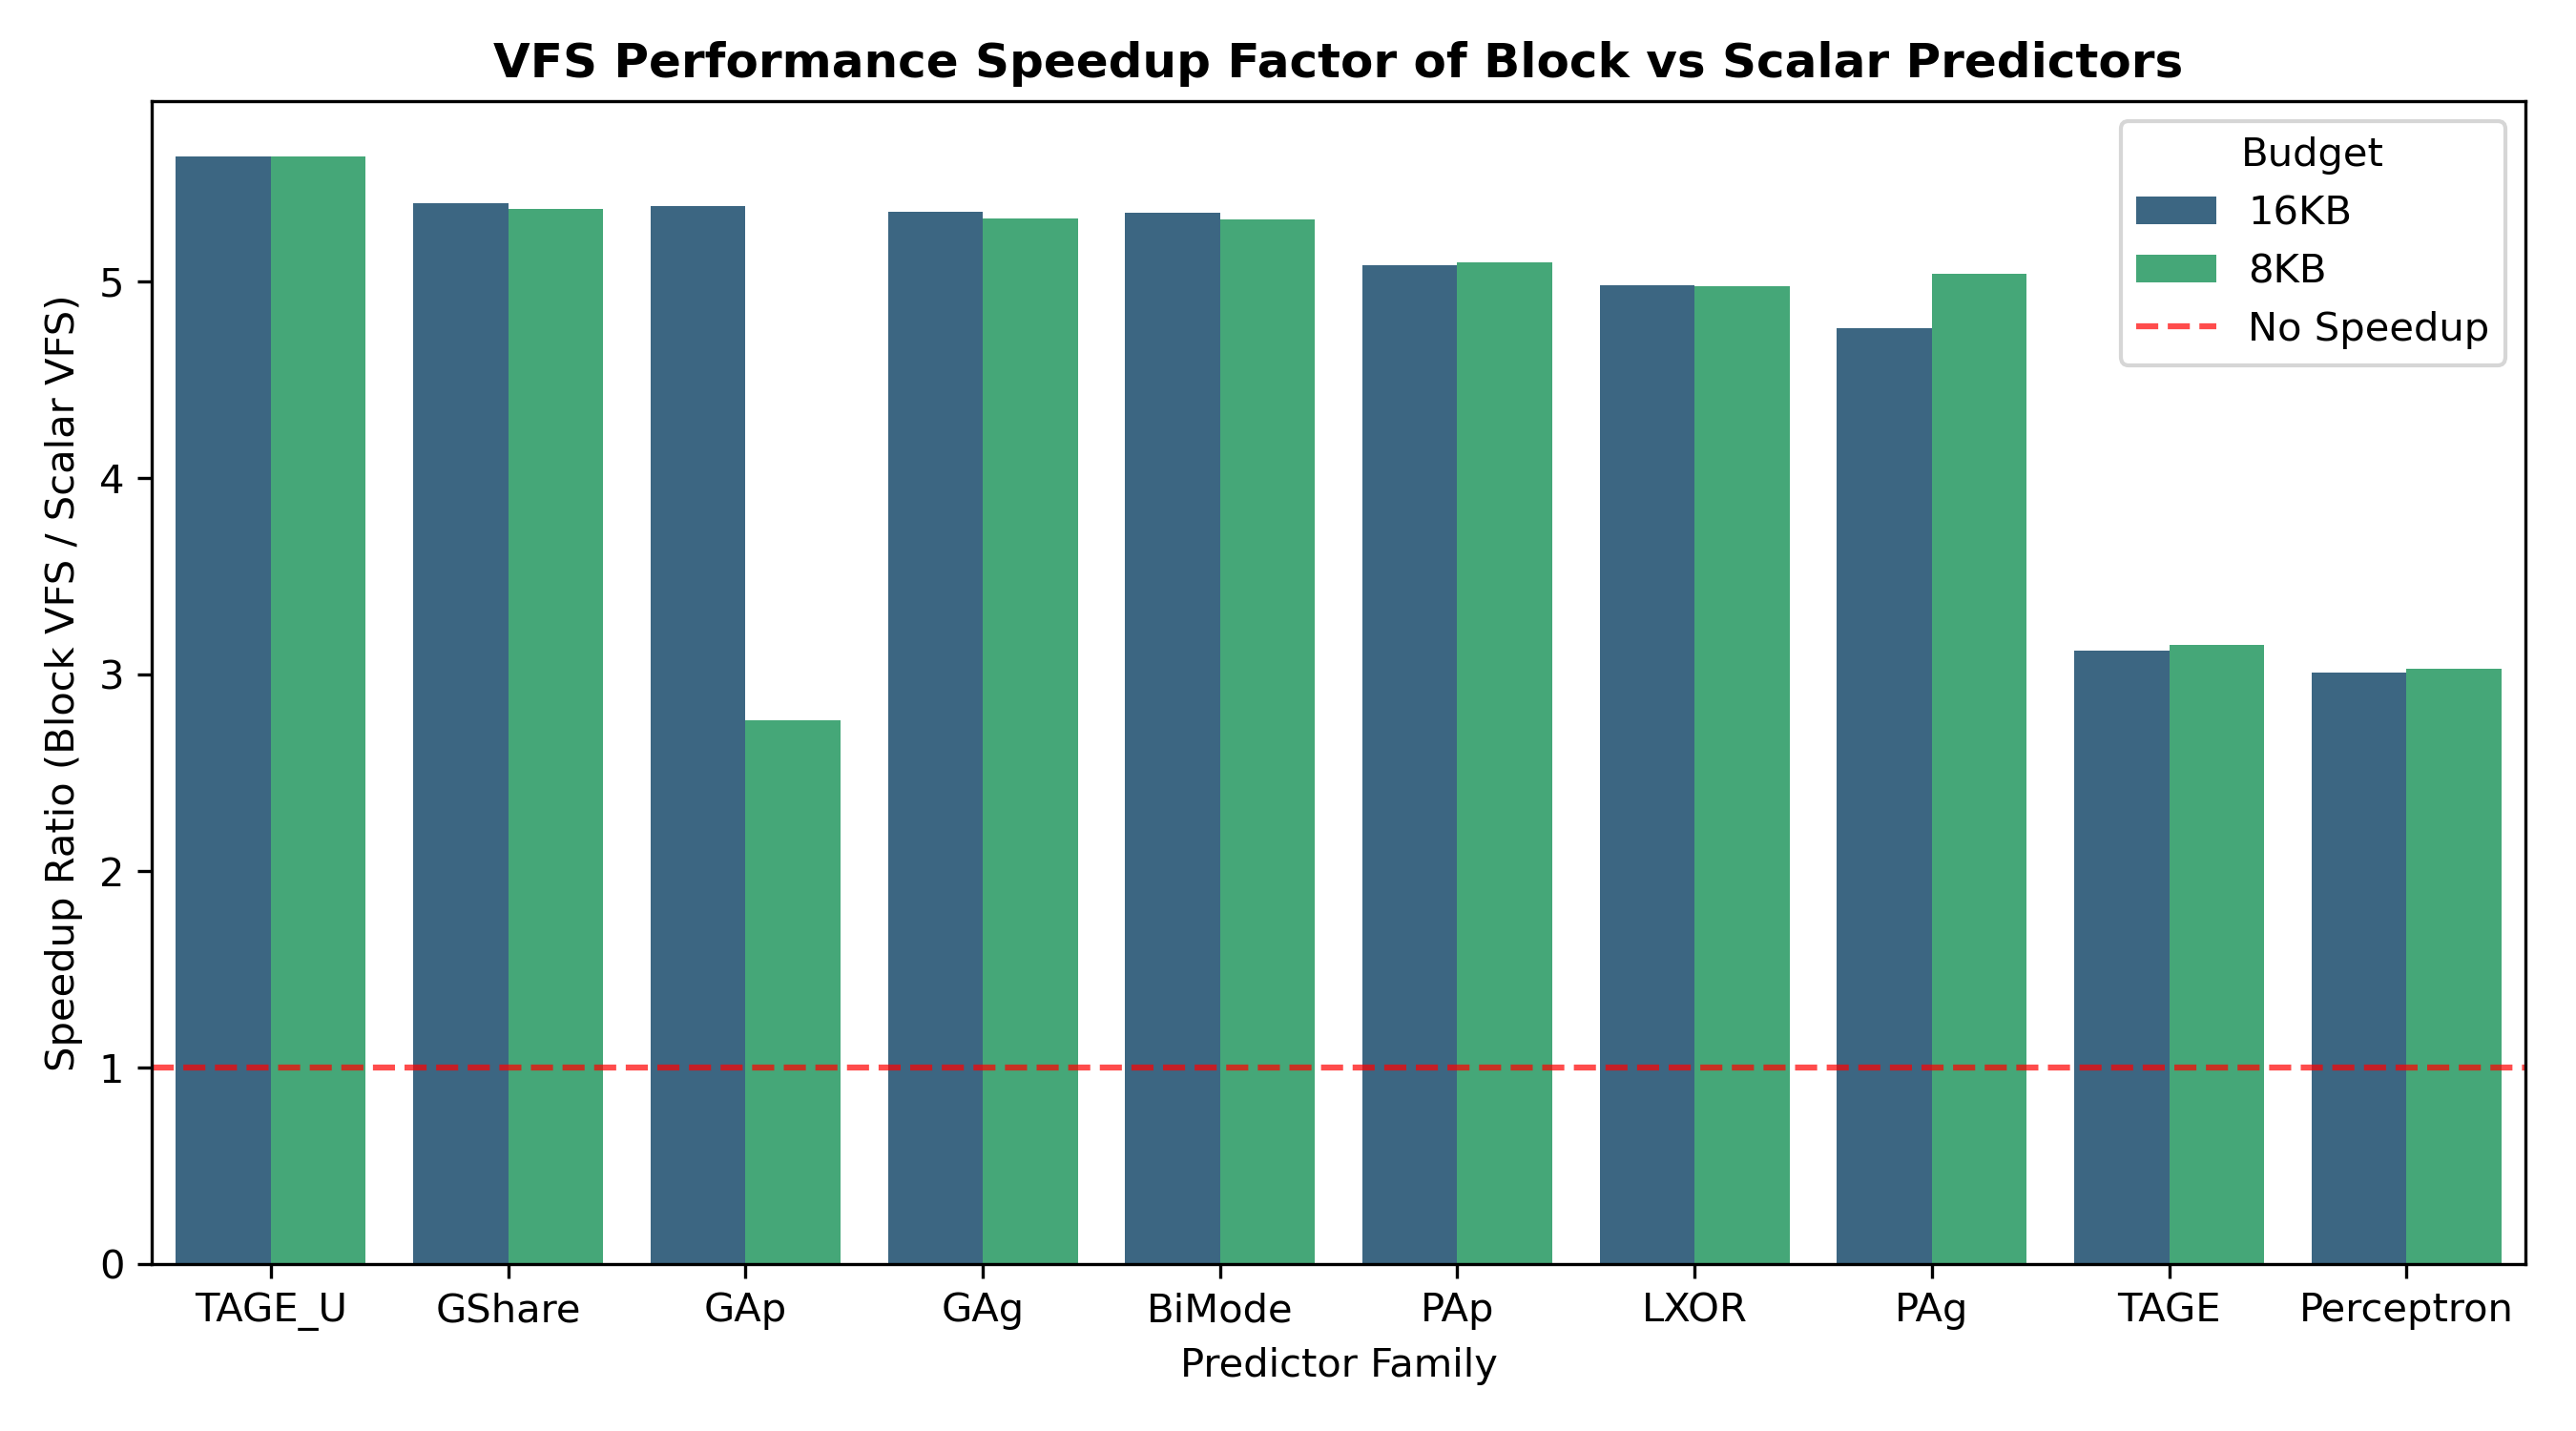
\includegraphics[width=1\linewidth]{family_speedup}
    \caption{\textbf{VFS Performance Speedup Factor of Block vs. Scalar Predictors.}}
    \label{fig:family_speedup}
\end{figure}

%---------------------------------------------------------------------------
%  BIBLIOGRAPHY
%---------------------------------------------------------------------------
\nocite{kise2005bimode}
\nocite{sutar2025towards}
\bibliography{bibliography.bib}

\end{document}
